\chapter{Ugeopgave 6}
\label{sec:ugeopgave-6}

Form�let med denne ugeopgave var at blive bekendt med OpenGL's
interface til \emph{vertex}- og \emph{fragmentshadere} samt
\emph{shading}-sproget GLSL.

\section{Del 1}
\label{sec:del-1-1}

Scenen, tegnet med OpenGL's normale \emph{pipeline} kan ses p� figur
\ref{fig:6-1}. I programmet blev linjen, der aktiverede
\emph{shaderne} udkommenteret, hvormed OpenGL selv s�rgede for
\emph{shading} af tepotten.

\begin{figure}[hp]
\centering
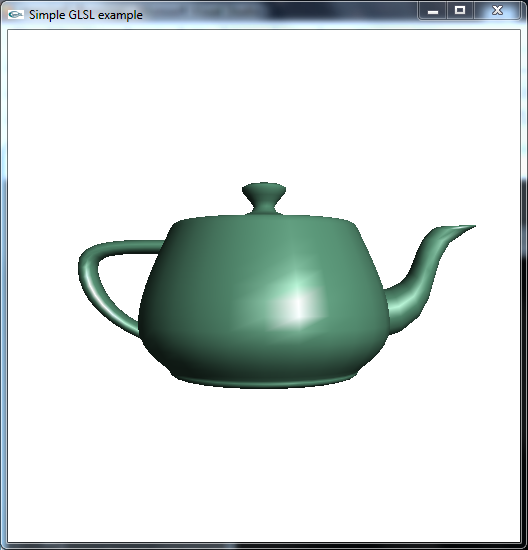
\includegraphics[width=8cm]{../exercise6/screenshots/part1.png}
\caption{OpenGL's normale pipeline}
\label{fig:6-1}
\end{figure}

\section{Del 2}
\label{sec:del-2-1}

Vha. de f�lgende to shaderprogrammer, blev Gouraud-shading
implementeret i GLSL:

\begin{verbatim}
// Vertex shader
void main()
{
  gl_Position = ftransform();

  vec4 ambient;
  vec4 diffuse;
  vec4 specular;
  vec4 eyePosition = gl_ModelViewMatrix * gl_Vertex;
  vec4 eyeLightPos = gl_LightSource[0].position;
  vec3 N = normalize(gl_NormalMatrix * gl_Normal);
  vec3 L = normalize(eyeLightPos.xyz - eyePosition.xyz);
  vec3 E = -normalize(eyePosition.xyz);
  vec3 H = normalize(L + E);
  float Kd = max(dot(L, N), 0.0);
  float Ks = pow(max(dot(N, H), 0.0), gl_FrontMaterial.shininess);
  float Ka = 0.2;

  ambient = Ka*gl_FrontLightProduct[0].ambient;
  diffuse = Kd*gl_FrontLightProduct[0].diffuse;
  specular = Ks*gl_FrontLightProduct[0].specular;
  gl_FrontColor = ambient+diffuse+specular;
}
\end{verbatim} \\

\begin{verbatim}
// Fragment shader
void main()
{
    gl_FragColor = gl_Color;
}
\end{verbatim}

Resultatet kan ses p� figur \ref{fig:6-2}.

\begin{figure}[hp]
\centering
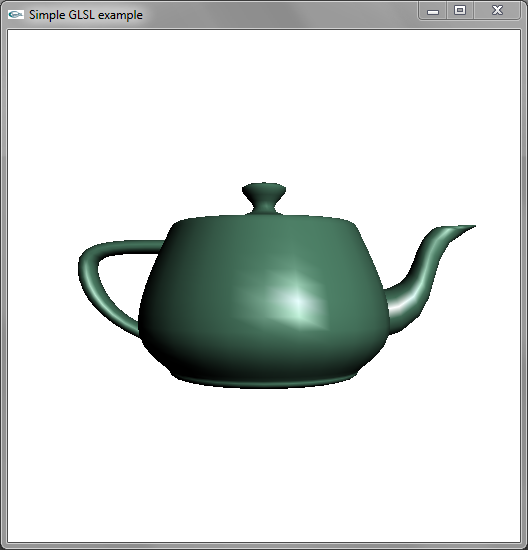
\includegraphics[width=8cm]{../exercise6/screenshots/part2.png}
\caption{Per-vertex Gouraud-shading i GLSL}
\label{fig:6-2}
\end{figure}

\section{Del 3}
\label{sec:del-3-1}

Her skulle per-vertex shadingen fra forrige delopgave erstattes med
per-fragment shading, dvs. Phong-shading.

Det blev gjort vha. f�lgende to shaderprogrammer:

\begin{verbatim}
// Vertex shader
varying vec3 N;
varying vec3 L;
varying vec3 E;
varying vec3 H;

void main()
{
  gl_Position = ftransform();

  vec4 eyePosition = gl_ModelViewMatrix * gl_Vertex;
  vec4 eyeLightPos = gl_LightSource[0].position;

  N = normalize(gl_NormalMatrix * gl_Normal);
  L = normalize(eyeLightPos.xyz - eyePosition.xyz);
  E = -normalize(eyePosition.xyz);
  H = normalize(L + E);
}
\end{verbatim} \\

\begin{verbatim}
// Fragment shader
varying vec3 N;
varying vec3 L;
varying vec3 E;
varying vec3 H;

void main()
{
  vec3 Normal = normalize(N);
  vec3 Light  = normalize(L);
  vec3 Eye    = normalize(E);
  vec3 Half   = normalize(H);

  float Kd = max(dot(Normal, Light), 0.0);
  float Ks = pow(max(dot(Half, Normal), 0.0), gl_FrontMaterial.shininess);
  float Ka = 0.2;

  vec4 diffuse  = Kd * gl_FrontLightProduct[0].diffuse;
  vec4 specular = Ks * gl_FrontLightProduct[0].specular;
  vec4 ambient  = Ka * gl_FrontLightProduct[0].ambient;

  gl_FragColor = diffuse + specular + ambient;
}
\end{verbatim}

Resultatet kan ses p� figur \ref{fig:6-3}.

\begin{figure}[hp]
\centering
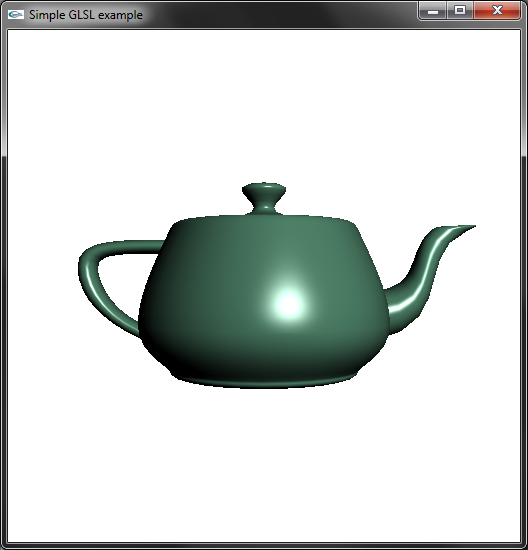
\includegraphics[width=8cm]{../exercise6/screenshots/part3.png}
\caption{Per-fragment Phong-shading i GLSL}
\label{fig:6-3}
\end{figure}

%%% Local Variables: 
%%% mode: latex
%%% TeX-master: "report_main"
%%% End: 